\documentclass[11pt]{article}
    \usepackage{caption}
    \usepackage{graphicx}
    \usepackage{mathtools}
    \graphicspath{ {img/} }
    \setlength{\parindent}{0pt}
    \DeclareCaptionType{equ}[][]
    \usepackage[svgnames]{xcolor}
    
    \newcommand*{\plogo}{\fbox{$\mathcal{BM}$}}
        
    \usepackage{PTSerif}
    
    \begin{document} 
        
    \begin{titlepage}
    
        \raggedleft
        
        \vspace*{\baselineskip}
        
        {\Large Bryan Melanson}
        
        \vspace*{0.167\textheight}
        
        \textbf{\LARGE How to Not Fail}\\[\baselineskip]
        
        {\textcolor{Red}{\Huge Electronic Circuits II}}\\[\baselineskip]
        
        {\Large \textit{While never going to class}}
        
        \vfill
        
        {\large Computer Engineering 2020 ~~\plogo}
        
        \vspace*{3\baselineskip}
    
    \end{titlepage}

    \pagebreak
    
%%%%%%%%%%%%%%%%%%%%%%%%%%%%%%%%%%%%%%%%%%%%%%%%%
    \tableofcontents

    \pagebreak
%%%%%%%%%%%%%%%%%%%%%%%%%%%%%%%%%%%%%%%%%%%%%%%%%

    
    \section{Operational Amplifiers}
    An \textit{Operation Amplifier} is a device which, when powered by $+V$ and $-V$ DC power sources, will amplify an input signal with infinite gain. The input terminals are known as the \textit{non-inverting} ($+$) and \textit{inverting} ($-$) terminals.

    Where no input current enters $+$ and $-$, and the \textit{input impedance is infinite.}

    \begin{figure}[h]
        \centering
        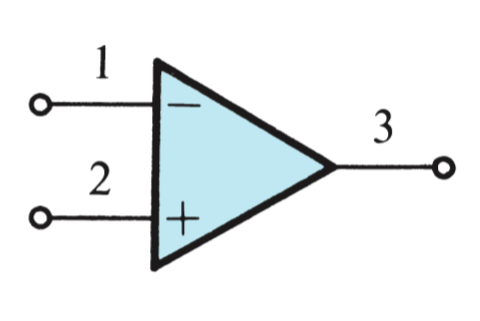
\includegraphics[width=\textwidth]{op}
        \caption{Ideal Op Amp}
        \label{fig:op amp}
    \end{figure}

    $A$ is referred to as the \textbf{Open Loop Gain}, where the output and inputs have not been connected. The \textbf{Closed Loop Gain} will be denoted as $G$. \\ 

    The \textbf{Differential Input Signal} $v_{id}$ and \textbf{Common Mode Input Signal} $v_{Icm}$ are two signals that define the operation of the op-amp. Because the op-amp is designed to detect the difference between two signals, they are denoted as the term $v_id$. The op-amp will also reject common signals, because only the difference between the two signals will be used for output.

    \begin{center}
        $v_{id} = v_2 + v_1$ \\
        $v_{Icm} = \frac{1}{2}(v_1 + v_2)$ 
    \end{center}

    \subsection{Inverting Configuration}

    In the inverting configuration, the output of the op-amp is connected back into the inverting terminal. Because in the inverting configuration $v_2$ is grounded, the negative output counteracts the inifite gain and \textit{closes the loop} around the op amp so that it provides a stable output. \\
    
    In the case where a resistance is placed between $v_2$ and $v_o$, there would be a \textbf{Positive Feedback}, and the output would increase exponentially.
   
    \begin{figure}[h]
        \centering
        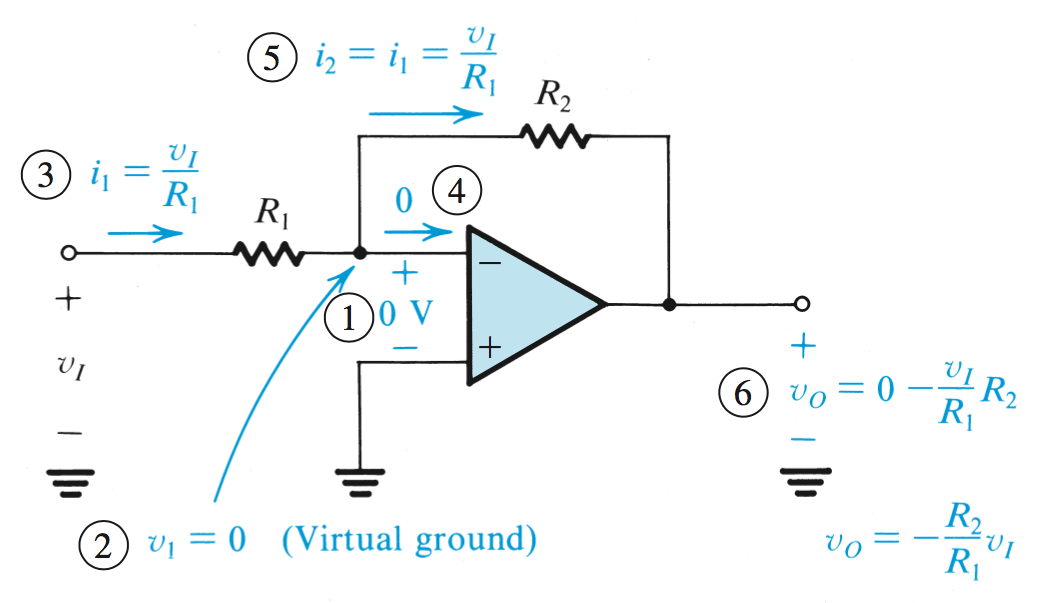
\includegraphics[width=\textwidth]{invert}
        \caption{Inverting Configuration of Op Amp}
        \label{fig:inverting }
    \end{figure}

    \begin{center}
        $v_3 = A(v_2-v_1)$
    \end{center}

    If $v_2 = v_1$, the output will be $0$. Where A is infinite,

    \begin{center}
        $\frac{v_3}{A} = v_2-v_1$ \\
        
        $0 = v_2-v_1$

        $v_2 = v_1$
    \end{center}

    This is known as a \textit{Virtual Short Circuit}. \\
    
    The \textbf{Closed Loop Gain} $G$ is defined as $\frac{v_o}{v_i}$ \\
    
    From Figure 1, we can see that knowing $v_1 = v_2 = 0$, therefore $i_1$ can be calculated, and passes to the input without entering the op amp terminals. \\
    
    \begin{equ}[!ht]
        \begin{equation}
            G = \frac{v_0}{v_i} = -\frac{R_2}{R_1}
        \end{equation}
      \caption{Closed Loop Gain of a Non-Inverting Amplifier}
    \end{equ} 
    
    \subsubsection{Finite Open-Loop Gain}
    When the open-loop gain $A$ is not finite, $\frac{v_3}{A} = v_2-v_1$ no longer produces $v_2 = v_1 = 0$, instead $v_2 = v_1 = \frac{v_o}{A}$. Knowing this, calculations for $i_1$ will follow the same logic, instead with accounting for $\frac{v_0}{A}$.
    \subsubsection{Input and Output Resistance}
    The input resistance is equal to $R_1$, and the output resistance is $0$.
    \subsubsection{Weighted Summer}
    In this configuration, $i$ will be the sum of all incoming currents. Therefore, 
    
    \begin{center}
        $i = \frac{v_1}{R_1} + \frac{v_2}{R_2} + ...$ \\
    \end{center}

    In the case where a design must be created to fit an equation with multiple inverted signs, two op-amps can used in series to flip the initial signals.

    \begin{center}
        $v_o = v_1(\frac{R_a}{R_1})(\frac{R_c}{R_b}) + v_2(\frac{R_a}{R_2})(\frac{R_c}{R_b}) - v_3(\frac{R_c}{R_3}) - v_4(\frac{R_c}{R_4})$
    \end{center}

    \begin{figure}[h]
        \centering
        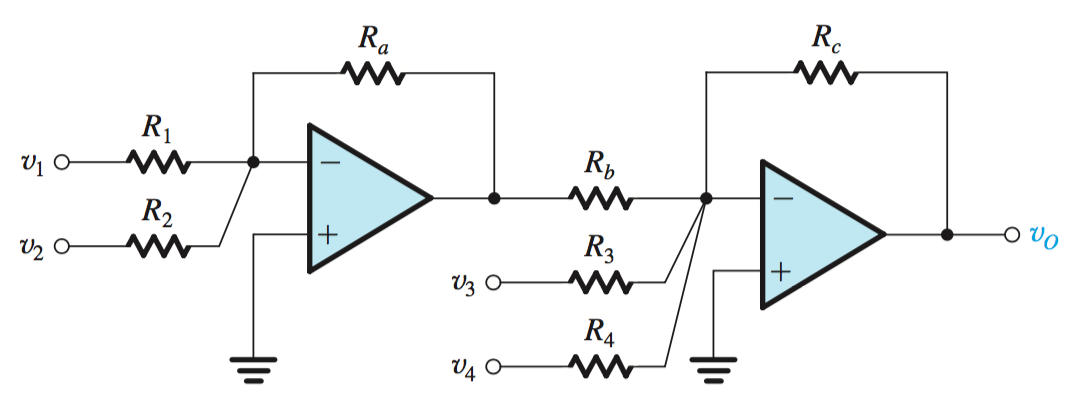
\includegraphics[width=\textwidth]{summer-2}
        \caption{Weighted Summers in Series}
        \label{fig:weight summers}
    \end{figure}

    \subsection{Non-Inverting Configuration}

    The Non-inverting configuration occurs when a voltage input enters the $v_2$ terminal, instead of $v_1$, while the resistor loop configuration is identical. As with the other closed loop, there is a virtual short circuit between $v_2$ and $v_1$, therefore $v_2 = v_1 = v_I$, the applied voltage. \\
    
    The $v_1$ terminal, grounded in this case, creates $i_1 = \frac{v_I}{R_1}$, and the solution can follow as before.

    \begin{equ}[!ht]
        \begin{equation}
            G = \frac{v_0}{v_i} = 1 + \frac{R_2}{R_1}
        \end{equation}
      \caption{Closed Loop Gain of a Non-Inverting Amplifier}
    \end{equ}
    
    \subsubsection{Finite Open-Loop Gain}

    When the open-loop gain $A$ is not finite, $\frac{v_3}{A} = v_2-v_1$ no longer produces $v_2 = v_1 = 0$, instead $v_2 = v_1 = \frac{v_o}{A}$. Knowing this, calculations for $i_1$ will follow the same logic, instead with accounting for $\frac{v_0}{A}$.

    \subsubsection{Buffering Amplifier or Voltage Follower}
    
    In this configuration, the loop is closed by short circuiting the output to non-inverting input. This will again create a virtual short circuit between $v_2$ and $v_1$, and because a real short circuit exists between $v_1$ and $v_o$, all terminal values will be equal to the voltage source, $v_I$. \\
    
    \begin{figure}[h]
        \centering
        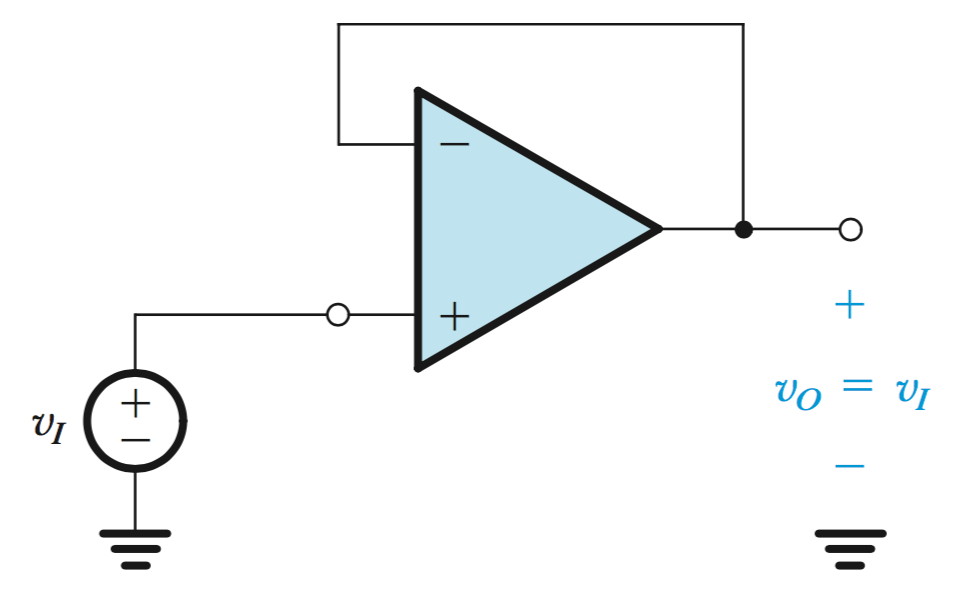
\includegraphics[width=\textwidth]{buff}
        \caption{Buffer Amplifier or Voltage Follower}
        \label{fig:voltage follower}
    \end{figure}

    \subsection{Difference Amplifiers}
    A Difference Amplifier is one where voltage sources are applied to the $v_2$ and $v_1$ inputs. The output can then be considered a non-inverting configuration and an inverting configuration superimposed on each other. By using supoerposition, the effect of each voltage source can then be calculated separately and summed together independent of one another. \\

    In a case like this, $v_o = A_dv_{id} + A_{cm}v_{Icm}$, and the efficiency of the Difference Amplifier can be determined by its \textit{common-mode rejection ratio (CMRR)}

    \begin{equ}[!ht]
        \begin{equation}
            \text{CMRR} = 20 \text{log}\frac{|A_d|}{|A_{cm}|}
        \end{equation}
      \caption{Common Mode Rejection Ratio}
    \end{equ}

    In a Difference amplifier with voltage sources at $v_2$ and $v_1$, it can be seen that this will have a inverting and non-inverting output superimposed on one another. However, the gain ratio of both inputs must be equal for the common mode ratio rejection, so the $v_2$ input must use a voltage divider ($v_3$ and $v_4$) to reduce the input voltage.\\
    
    Therefore, $\frac{R_4}{R_4 + R_3}(1 + \frac{R2}{R1}) = \frac{R2}{R1}$, and $\frac{R4}{R3} = \frac{R2}{R1}$. \\

    To find values concering solely the $v_{Id}$ and $v_{Icm}$, consider a voltage source $v_Id$ or $v_Icm$ applied at the inputs, where $v_Icm$ is applied to both, and the negative and positve termals of $v_{id}$ are connected in series between the two terminals.

    \begin{figure}[h]
        \centering
        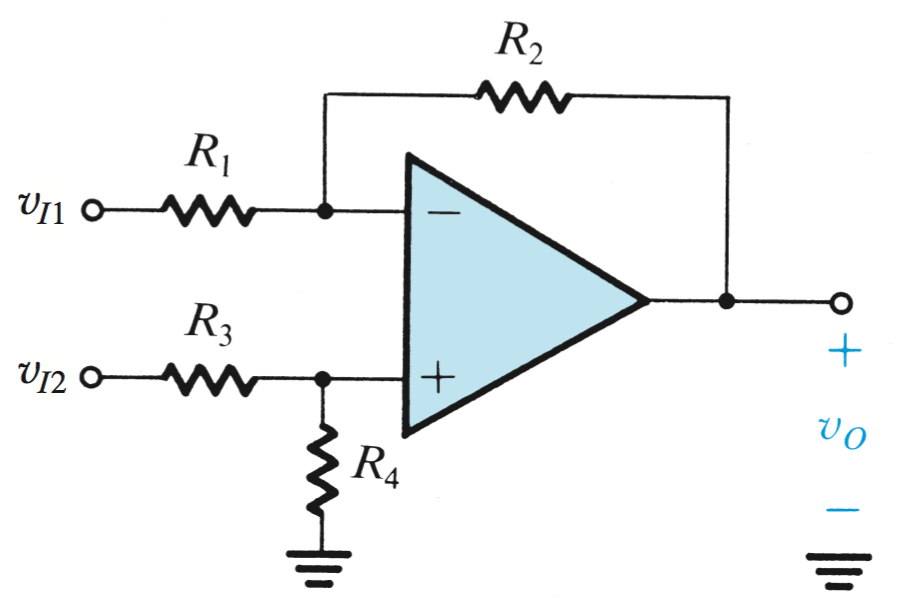
\includegraphics[width=\textwidth]{diff}
        \caption{Difference Amplifier}
        \label{fig:difference amplifier}
    \end{figure}

    \subsubsection{Instrumentation Bridge Amplifiers}

    The Instrumentation Bridge Amplifier is a Difference Amplifier created as a solution to the low input resistance of Difference Amplifiers, without sacrificing ease of control. From Figure 6, it can be noted that $R_1$ can be used to control the output voltage of the circuit.
    
    \begin{equ}[!ht]
        \begin{equation}
            v_o = \frac{R4}{R3}(1 + \frac{R_2}{R_1})v_{Id}
        \end{equation}
      \caption{Output of the Instrumentation Bridge Amplifier}
    \end{equ}

    \begin{figure}[h]
        \centering
        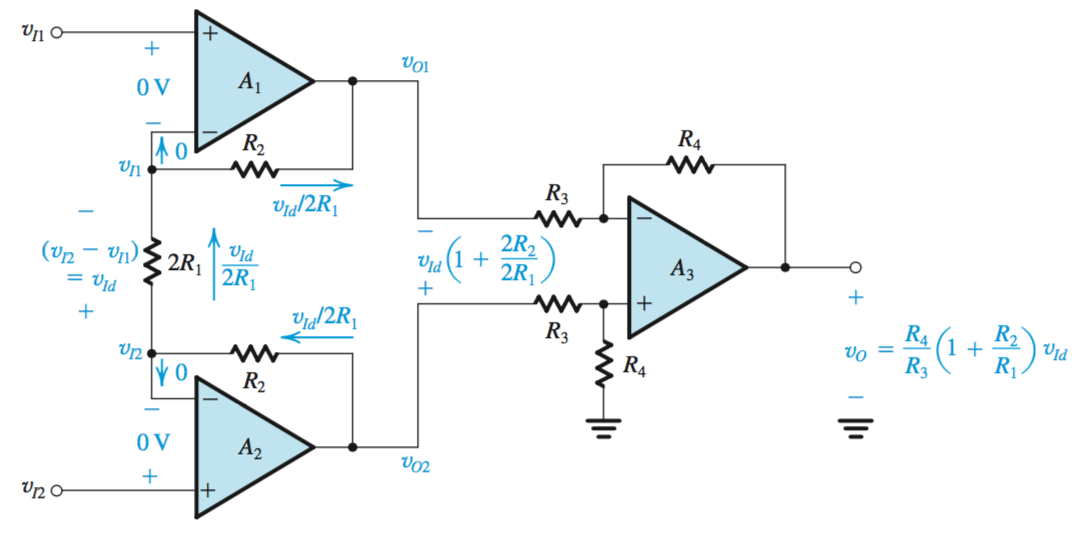
\includegraphics[width=\textwidth]{instr}
        \caption{Instrumentation Bridge Amplifier}
        \label{fig:instrumentation bridge amplifier}
    \end{figure}

%%%%%%%%%%%%%%%%%%%%%%%%%%%%%%%%%%%%%%%%%%%%%%%%%

    \section{Filters and Tuned Amplifiers}
    \subsection{Filter Transmission}
    \subsection{Filter Transmission (2nd Order Filters)}
    \subsection{Second Order LCR Resonator}
    \subsection{Second Order Active Filters}
    \subsection{Second Order Active Filters Based on Two Integrator Loop Topology}
    \subsection{Single Amplifier Biquadratic Active Filters}
    \subsection{Sensitivity}

%%%%%%%%%%%%%%%%%%%%%%%%%%%%%%%%%%%%%%%%%%%%%%%%%

    \section{Signal Generators and Waveform-Shaping Circuits}
    \subsection{Basic Principles of Sinusoidal Oscillators}
    \subsection{Bistable Multivibrators}
    \subsection{Op Amp RC Oscillator Circuits}
    \subsection{Generation Waveforms Using Astable Multivibrators}
    \subsection{Generation of a Standardized Pulse: The Monostable Multivibrator}
    \subsection{Precision Rectifiers}

    \end{document}